\begin{figure}[H]
	\begin{center}
		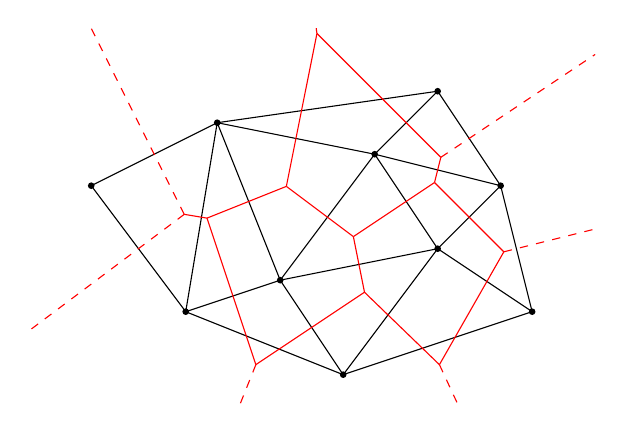
\begin{tikzpicture}[scale=0.4]
		%\draw [<->,thick] (0,10) node (yaxis) [left] {}
		%|- (15,0) node (xaxis) [below] {};
		%centroids
		\fill ( 2, 7) circle (3pt);
		\fill ( 5, 3) circle (3pt);
		\fill ( 6, 9) circle (3pt);
		\fill ( 8, 4) circle (3pt);
		\fill (10, 1) circle (3pt);
		\fill (11, 8) circle (3pt);
		\fill (13, 5) circle (3pt);
		\fill (13,10) circle (3pt);
		\fill (15, 7) circle (3pt);
		\fill (16, 3) circle (3pt);
		
		%DELAUNAY
		\draw [-] ( 2,7) -- ( 6,9);
		\draw [-] ( 6,9) -- ( 5,3);
		\draw [-] ( 5,3) -- ( 2,7);
		\draw [-] ( 6,9) -- ( 8,4);
		\draw [-] (10,1) -- ( 8,4);
		\draw [-] ( 5,3) -- (10,1);
		\draw [-] ( 8,4) -- ( 5,3);
		\draw [-] ( 8,4) -- (11,8);
		\draw [-] (11,8) -- (6,9);
		\draw [-] ( 6,9) -- (13,10);
		\draw [-] (11,8) -- (13,10);
		\draw [-] (15,7) -- (13,10);
		\draw [-] (16,3) -- (15,7);
		\draw [-] (16,3) -- (10,1);
		\draw [-] (16,3) -- (13,5);
		\draw [-] (13,5) -- (15,7);
		\draw [-] (13,5) -- (10,1);
		\draw [-] (13,5) -- (8,4);
		\draw [-] (13,5) -- (11,8);
		\draw [-] (15,7) -- (11,8);
		
		%VORONOI		
		\draw [-,red] ( 5.6764, 5.9706) -- ( 4.9545, 6.0909);
		\draw [-,red] ( 5.6764, 5.9706) -- ( 8.1956, 6.9783);
		\draw [-,red] (10.3235, 5.3824) -- ( 8.1956, 6.9783);
		\draw [-,red] (10.3235, 5.3824) -- (10.6765, 3.6176);
		\draw [-,red] ( 7.2272, 1.3182) -- (10.6765, 3.6176);
		\draw [-,red] ( 7.2272, 1.3182) -- ( 5.6764, 5.9706);
		\draw [-,red] (13.0556, 1.3182) -- (10.6765, 3.6176);
		\draw [-,red] (13.0556, 1.3182) -- (15.1000, 4.9000);
		\draw [-,red] (12.9000, 7.1000) -- (15.1000, 4.9000);
		\draw [-,red] (12.9000, 7.1000) -- (10.3235, 5.3824);
		\draw [-,red] (12.9000, 7.1000) -- (13.1000, 7.9000);
		\draw [-,red] ( 9.1667,11.8333) -- (13.1000, 7.9000);
		\draw [-,red] ( 9.1667,11.8333) -- ( 8.1956, 6.9783);
		
		\draw [-,red,dashed] ( 4.9545, 6.0909) -- (	2.0000,12.0000);
		\draw [-,red,dashed] ( 4.9545, 6.0909) -- (	0.0000,	2.3750);
		\draw [-,red,dashed] ( 7.2272, 1.3182) -- (	6.7000, 0.0000);
		\draw [-,red,dashed] (13.0556, 1.3182) -- (13.6667, 0.0000);
		\draw [-,red,dashed] (15.1000, 4.9000) -- (18.0000, 5.6250);
		\draw [-,red,dashed] (13.1000, 7.9000) -- (18.0000,11.1667);
		\draw [-,red,dashed] ( 9.1667,11.8333) -- ( 9.1429,12.0000);
		
		\end{tikzpicture}
	\end{center}
	\caption{Overlap of a Voronoi Diagram and its Delaunay Triangulation}
	\label{fig:dt_vd}
\end{figure}